\documentclass{article}
\usepackage{graphicx,wrapfig,lipsum}
\usepackage[utf8]{inputenc}

\title{Progettazione di una base di dati per esperimenti scientifici}
\author{Francesco Andreuzzi - IN0500630}
\date{\today}

\renewcommand{\figurename}{Fig.}

\begin{document}
\maketitle

Durante lo sviluppo di un progetto scientifico che comporti l'esecuzione di esperimenti di lunga durata che producano un output non banale, mantenere ordine tra i dati disponibili diventa rapidamente complesso e dispendioso in termini di tempo. Il proliferare dei metodi sperimentati (nell'\hphantom{xcjxxsksjskksksk}
\begin{wrapfigure}{r}{2cm}
    \vspace{-0.9cm}
    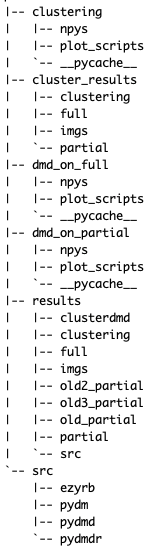
\includegraphics[width=2cm]{res/tree_brutto.png}
    \caption{\texttt{tree} della directory di un progetto.}\label{fig:tree}
\end{wrapfigure}
{ambito dello stesso progetto) al fine di pervenire all'obiettivo preposto, eventualmente insieme all'aumentare del numero di parametri che controllano determinate caratteristiche degli stessi, rende la situazione ancora più caotica.  Il progetto si propone il compito di risolvere questo problema con una base di dati, al fine di evitare gerarchie di cartelle con cui risulta difficoltoso lavorare a lungo termine (come quella in Figura \ref{fig:tree}).\par}

\section{Entità}
Nel progetto saranno utilizzate le seguenti entità, ognuna rappresentata da una tabella:
\begin{itemize}
    \item Dataset \begin{itemize}
        \item \emph{ID};
        \item \emph{Format};
        \item \emph{Notes}.
    \end{itemize}
    \item Algorithm \begin{itemize}
        \item \emph{ID};
        \item \emph{Git-Branch};
        \item \emph{Requirements}.
        \item \emph{Notes}.
    \end{itemize}
    \item Parameters \begin{itemize}
        \item \emph{ID};
        \item \emph{Tuple};
    \end{itemize}
    \item Run \begin{itemize}
        \item \emph{ID};
        \item \emph{Date};
        \item \emph{Hardware-ID};
        \item \emph{Algorithm-ID};
        \item \emph{Dataset-ID};
        \item \emph{Parameters-ID};
        \item \emph{Outcome-ID};
    \end{itemize}
    \item Hardware \begin{itemize}
        \item \emph{ID};
        \item \emph{Label};
        \item \emph{Modules}
        \item \emph{Notes};
    \end{itemize}
    \item Outcome \begin{itemize}
        \item \emph{ID};
        \item \emph{Run-ID};
    \end{itemize}
\end{itemize}

\begin{figure}
    \makebox[\textwidth][c]{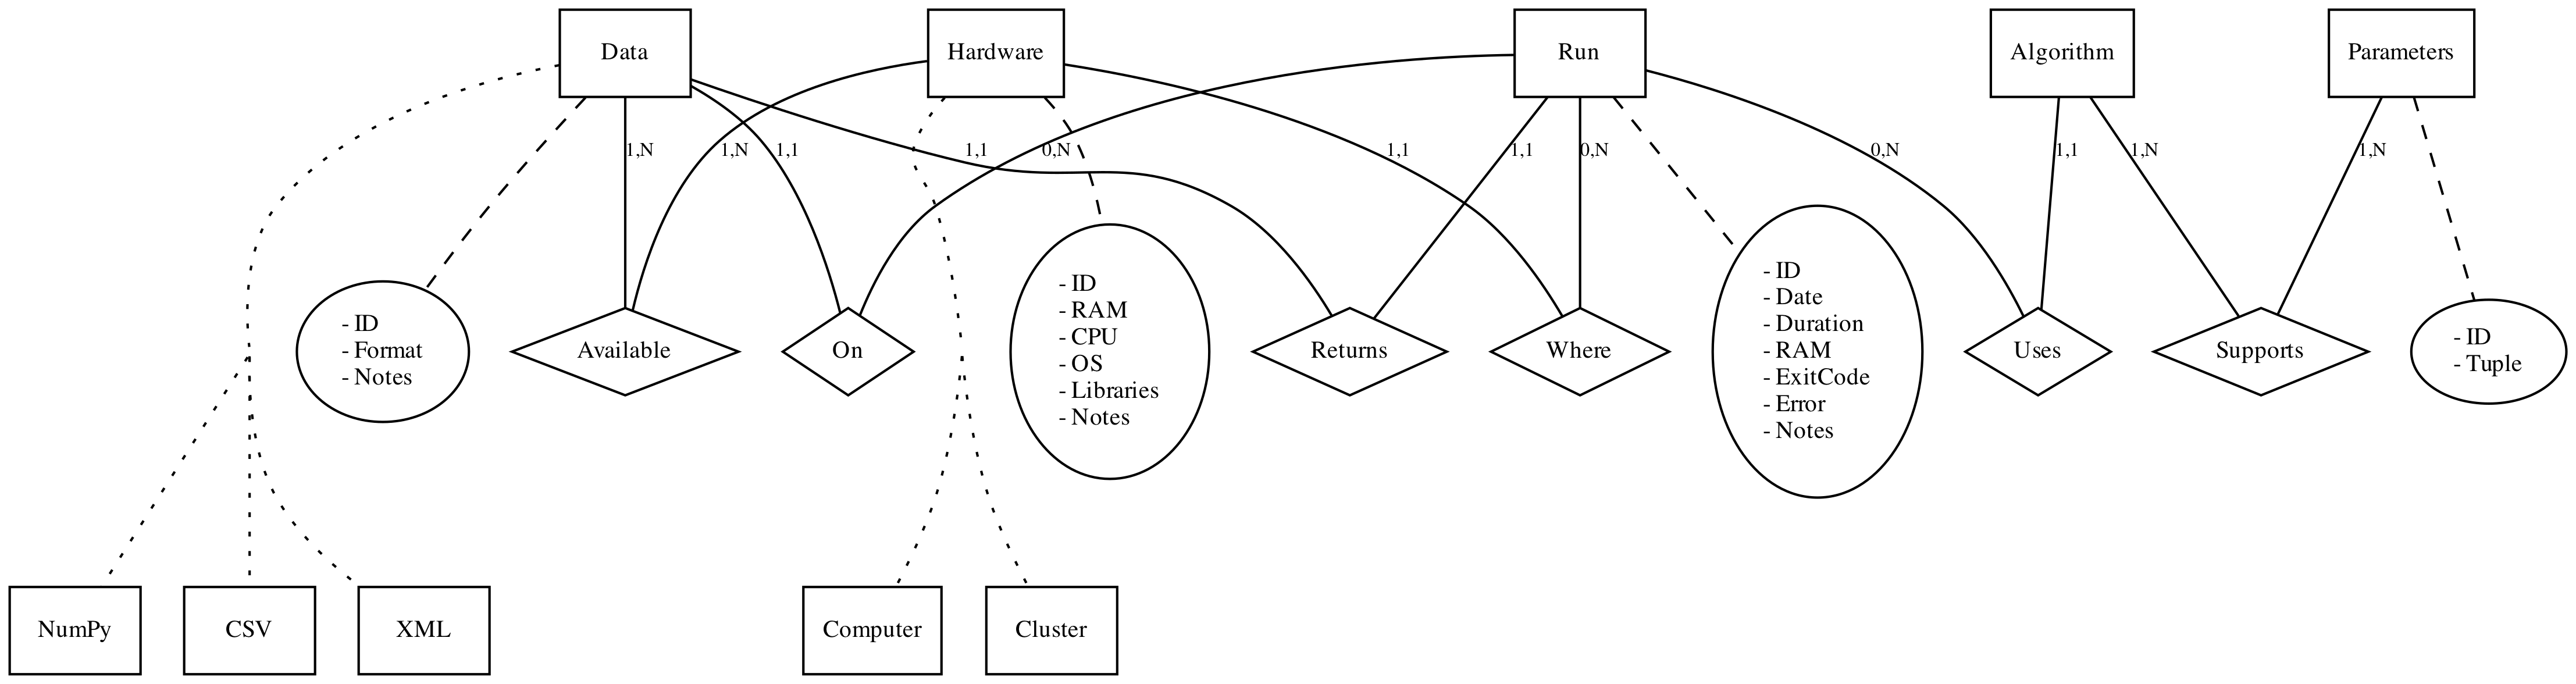
\includegraphics[width=1.6\textwidth]{res/schema_concettuale.png}}
    \caption{Schema concettuale del progetto.}
  \end{figure}

\section{Operazioni previste}

\section{Note}
In un contesto più realistico l'algoritmo dovrebbe essere un eseguibile, ma linguaggi come python non funzionano così. Dovrebbe essere previsto uno script di supporto.

Questo documento è stato realizzato con \LaTeX. Gli schemi sono stati realizzati in Python utilizzando le librerie \emph{NetworkX, (Py)Graphviz}, ed il VCS \emph{git}.

L'idea per questo progetto è stata ispirata dalla collera conseguente alla necessità di dover eseguire da zero un pool di 400 \emph{jobs} sul cluster HPC della SISSA perchè i risultati corrispondenti erano stati sovrascritti da un altro esperimento con un algoritmo diverso ma parametri identici.

\end{document}
